\section{Introduction}
The last several years have seen the emergence of programmable network devices including both programmable switching chips and programmable network interface cards (NICs). Along with the rise of x86-based packet processing for middleboxes and virtual switches, these trends point towards a future where the entire network will be programmable. The benefits of network programmability range from commercial use cases such as network virtualization implemented on Open vSwitch to more recent projects that implement packet scheduling, measurement, and application offload of niche applications on programmable switches. \\
\indent While the benefits of programmability are clear, it is still difficult to program the network as a whole. Current programming languages target individual network devices, e.g., P4 for the Tofino programmable switching chip and the Netronome programmable NIC. However, at present, there is no unified programming model to express and implement general functionality at the level of an entire network, without having to individually program each network device.\\
\indent Maple [39] was an early example of a network-wide programming model designed for OpenFlow switches. Maple automatically divided functionality between a stateless component running on switches and a stateful component running on the network's controller. SNAP [40] is a more recent example of network-wide programming; unlike Maple, it additionally offloads stateful functionality to switches by leveraging stateful processing available in several programmable switches. However, both Maple and SNAP cannot express programmable-switch functionality that affects network performance at fine time scales, e.g., packet scheduling, congestion control, fine-grained measurement of microbursts, and load balancing. For these reasons we have developed Sluice, a programming model that takes a high-level specification of a network program and compiles it into runnable code that can be launched on the programmable devices of network. Sluice endows network operators with the ability to design and deploy large network programs for various functions such as scheduling, measurement, and application offloading. We demonstrate Sluice's functionality and simplicity of use via two examples: traffic matrix generation for network analysis and a streaming join-filter operation.

\section{Sluice Design}
In the Sluice model, a network-wide program consists of high-level code \textit{snippets} annotated by the operator to run on particular devices in a network. The code in each snippet is to be executed on packets arriving at its corresponding device. Snippets support a variety of operations : read-from/write-to packets; arithmetic using packet data, local variables, or stateful register arrays; control flow statements. To handle computation on custom packet headers not supported by default (ip/tcp/udp/eth), users may define packet declarations similar to C structs. An optional annotation in the declaration, the parser condition, automatically generates a header parser. This lets the user restrict snippets to operate on specific flows or IP address ranges. Sluice programs may also import device-specific variables/attributes for use in code snippets. \\
\indent The compiler translates each snippet of a sluice program into a device-specific program. After initial parsing, a snippet is decomposed into a directed acyclic graph (DAG) that maps dependencies between variables in each snippet. This graph is then passed to the backend of the compiler that generates the corresponding P4 program for that device, for example bmv2 or Tofino \footnote{Currently we only support bmv2 but plan to support more devices}. Sluice automatically reduces the amount of boilerplate code needed to write an equivalent program in P4. For instance, the 9 line traffic matrix sluice program translates into over 200 lines of P4 code. Overall, Sluice provides the same functionality as P4 but makes it easier to program the data plane of an entire network


 
%Example of citation here\cite{floyd1993random, stoica2001chord}


\section{Demonstrations}
 
\subsection{Traffic Matrix}

\noindent Figure 2 displays the Mininet network topology and simulation components. Packets flow over UDP between virtual hosts, through a network of virtual programmable switches. The codelet in Figure 3 is a Sluice program with a single snippet 'traffic\_example' that is launched on all switches of the network. To run the simulation, the user passes the Sluice program and network topology to the compiler. The compiler generates P4 code to run on each switch as well as control plane table entries for routing packets through the topology.  \\
\indent This demo shows how a simple Sluice program can be used to program each switch to measure link usage and hop counts for a specific flow of user-defined packets on UDP srcPort 1234. Each packet 'p' contains a custom header 'nhops' that will be used by the host to maintain a time-series of hop counts. Specifically, nhops is incremented each time the packet enters a switch, i.e. on each hop. Each switch maintains a stateful register counter 'cnt', indexed by switch ingress port, that tracks how many packets, on the particular UDP flow 1234, have entered through that ingress port. Aggregated over all switches, these counters data represent a matrix measuring each link's usage in the network. This matrix (residing on the whole network) is then queried regularly from the control plane to generate time-series plots of link-utilization and queue depth.  

\begin{figure}[tp]
\centering
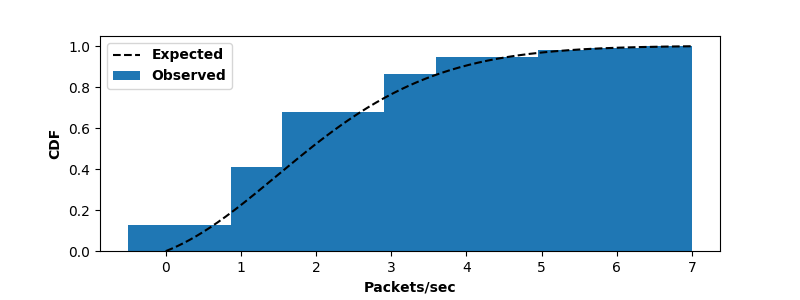
\includegraphics[width=80mm,scale=0.7]{figures/exp_obs_cdf}
\caption{Expected vs Observed Packet Rate CDF on ('s1','s2')}
\end{figure}


\begin{figure}[tp]
\centering
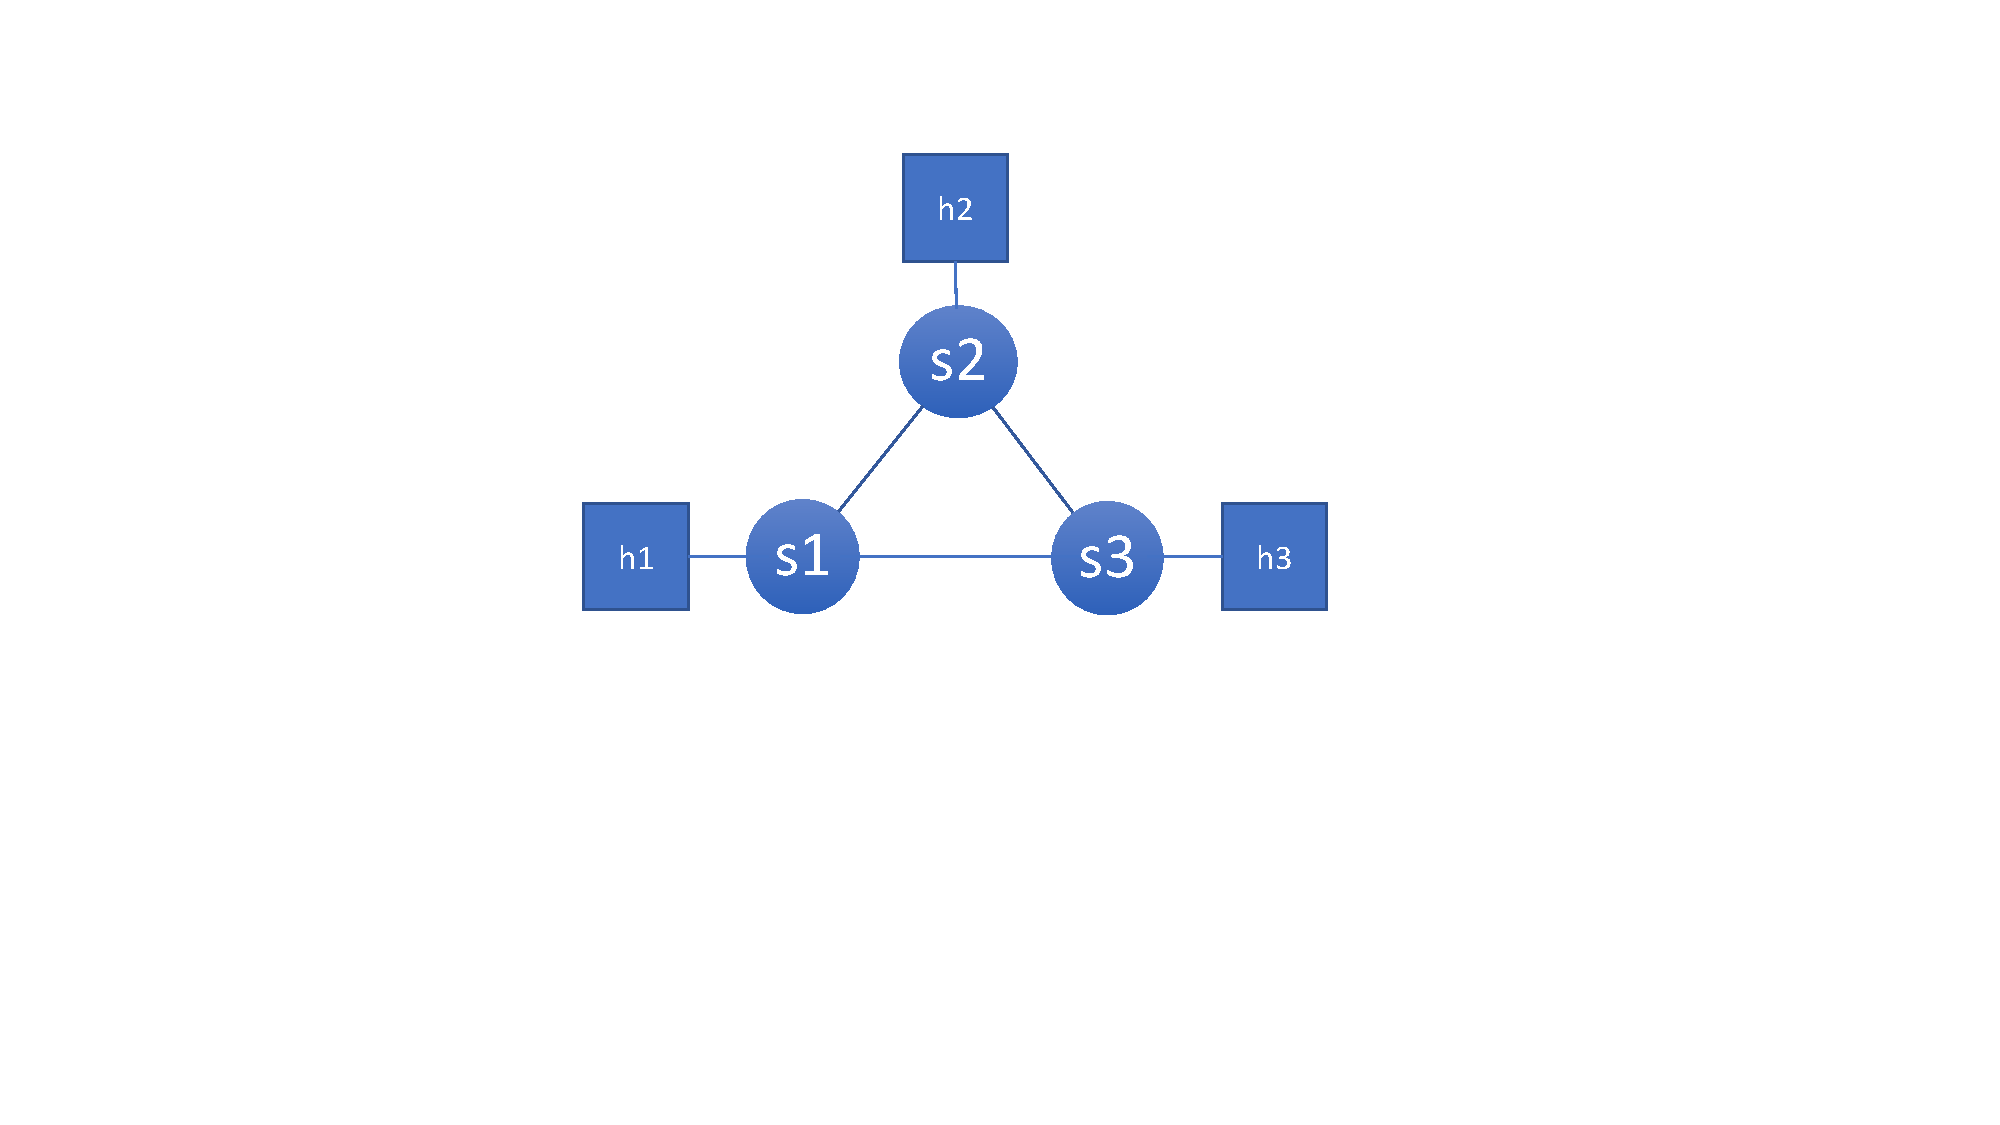
\includegraphics[width=40mm,scale=0.7]{figures/traf_mat_topo}
\caption{Topology For Traffic Matrix Demo}
\end{figure}

  
\subsection{Streaming Algorithms}
This example demonstrates a simple join-filter operation between two streams. A stream is an unbounded table where a packet represents a tuple of data (ad\_id, impression\_time, click\_time) enclosed in a custom header. The topology in Figure 4 describes the data flow and shows how an operator query runs on the switches of the network. Host 1 sends a stream of ad impressions while Host 2 sends a stream of ad clicks. The two streams are joined on the "ad\_id" field at s1 and filtered on the "ad\_id" field at s2 and the result is sent to h3. 


\section{Future Work}
We plan to focus on using the dependency DAG to provide several optimizations. For example, it is possible that certain lines of code in a snippet cannot be run on the device annotated by the operator. Since programmable switching chips do not support floating point or complex string operations, code containing such features must be moved to the control plane or end host while at the same time, preserving the original program semantics intended by the operator. The issue of code movement is particularly interesting in the context of multi-tenant data centers. Here, each tenant manages their own virtual network, which is mapped to physical nodes at the data center. If each tenant wants to run their own network-wide program on their virtual topology, the data center operator will need to merge all these into one data plane implementation that runs on the entire physical network. We will continue to develop Sluice with the hope that it may virtualize the data plane, in the same way as network virtualization virtualized the control plane.

\section{References}
